


\section{回顾:连续性}\label{ux56deux987eux8fdeux7eedux6027}

那么什么是Lipschitz连续呢,各种连续的关系又是什么呢,我们讨论的非连续动态微分方程又如何定义呢?
为了简便,这里用的是函数来叙述,实际控制理论中大多为多维到多维的向量函数。如果是多变量函数或者泛函需要使用范数替代绝对值。

可微必可导。
可微是可导的充分条件。
只不过在一元情况下,由于两点确定一条直线,导致可微的线性替代就相当于求导(斜率确定 点确定 相当于直线确定)

\subsection{点连续与间断点}

\begin{definition}[点连续]
设函数\(y=f(x)\)在点\(x_0\)的某一邻域内有定义,
并且\(\lim_{x\to x_0}f(x)=f(x_0)\),
那么就称函数\(f(x)\)在点\(x_0\)处连续。
\end{definition}

借此可以定义函数不连续和间断点的概念:
\begin{definition}
设函数\(f(x)\)在点\(x_0\)的某\textbf{去心}领域内有定义,
在此前提下,如果函数\(f(x)\)有一下三种情形之一 
\begin{enumerate}
  \item 在\(x=x_0\)处没有定义;
  \item 在\(x=x_0\)处有定义,但\(\lim_{x\to x_0} f(x)\)不存在;
  \item 在\(x=x_0\)处有定义,\(\lim_{x\to x_0} f(x)\)存在,但\(\lim_{x\to x_0}\neq f(x_0)\)
\end{enumerate}
那么函数\(f(x)\)在点\(x_0\)为不连续,\(x_0\)是函数\(f(x)\)的\textbf{间断点}。
\end{definition}



函数的间断点可以分为 
\begin{enumerate}
  \item 第一类间断点:左右极限都存在 
  \begin{enumerate}
    \item 可去间断点:左右极限都存在且相等 
    \item 跳跃间断点:左右极限都存在但不等 
  \end{enumerate}
  \item 第二类间断点:左右极限至少有一个不存在 
  \begin{enumerate}
    \item 震荡间断点:\(\lim_{x\to\ x_0} f(x)\)振荡不存在 
    \item 无穷间断点:\(\lim_{x\to\ x_0^+} f(x)=\infty\)或\(\lim_{x\to\ x_0^-} f(x)=\infty\)
  \end{enumerate}
\end{enumerate}


\begin{figure}[!hbp]
\centering
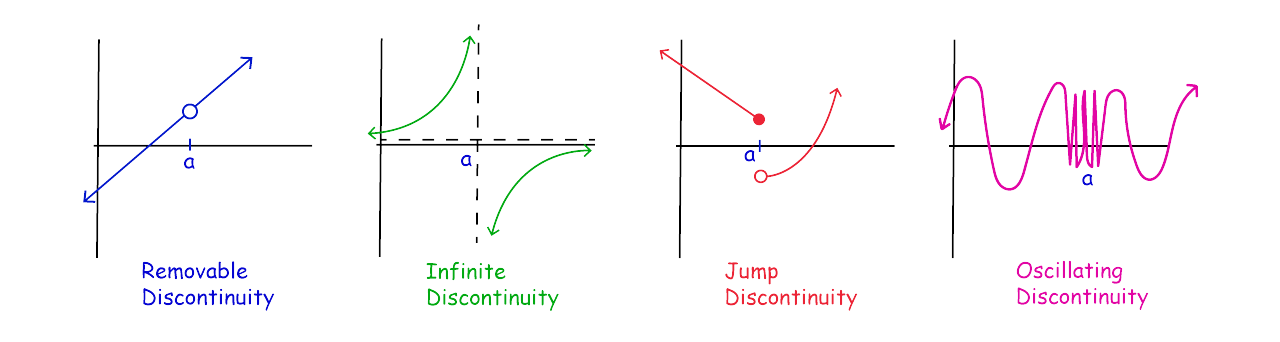
\includegraphics[width=\linewidth]{asserts/4-types-of-discontinuity.png}
\caption{
  间断点的定义与图示(来源:\url{https://calcworkshop.com/limits/limits-and-continuity/})
}
\end{figure}

\subsection{区间连续与区间一致连续(连续、绝对连续、Lipschitz连续、Hölder连续)}

如果在区间上每一点都连续,就称函数在该区间上连续,如果区间包括端点,那么在右端点连续是指左连续,在左端点连续是指右连续。

\begin{definition}[区间连续]
设函数\(f(x)\)在区间\(I\)上有定义.
如果对于任意给定的正数\(\epsilon\),总存在正数
\(\delta\),是的对于区间\(I\)上的任意两点\(x_1,x_2\),当\(|x_1-x_2|<\delta\)时,
有 \[
|f(x_1)-f(x_2)|<\epsilon
\] 那么称函数\(f(x)\)在区间\(I\)上\textbf{一致连续}。
\end{definition}

绝对连续表示函数的光滑性质,比连续和一致连续条件都要严格,比Lipschitz条件宽松,是一类极为重要的函数。绝对连续函数几乎处处可微,是它的导函数的广义原函数。

\begin{definition}[绝对连续]
设\(f(x)\)是\([a,b]\)上的函数,若对任意\(\epsilon>0\),存在\(\delta>0\)使得对于
\([a,b]\)中的任意一组分点: \[
a_1<b_1\leq a_2 <b_2 \leq \dots \leq a_n < b_n,
\] 只要\(\sum_{i=1}^n(b_i-a_i)<\delta\),便有 \[
\sum_{i=1}^n|f(b_i)-f(a_i)|<\epsilon
\]
则称\(f(x)\)是\([a,b]\)上\textbf{绝对连续}函数,或称\(f(x)\)在\([a,b]\)上绝对连续。
\end{definition}

等价的,如果存在一个Lebesgue可积函数\(\kappa:[a,b]\to \mathbb{R}\)
使得下式成立,那么\(\gamma\)是一个绝对连续函数。 \[
\gamma(t)=\gamma(a)+\int^t_a \kappa(s)d s,\quad t\in [a,b]
\]

\begin{definition}[Lipschitz连续]
对于函数\(f(x)\),如果存在一个常数L,使得对\(f(x)\)定义域上(可为实数也可以为复数)的任意两个值满足如下条件:
\[
|f(x_1)-f(x_2)|\leq L|x_1-x_2|
\]
那么称函数\(f(x)\)满足Lipschitz连续条件,并称L为\(f(x)\)的lipschitz常数。
\end{definition}

\begin{itemize}

\item
  从局部看:我们可以取两个充分接近的点,如果这个时候斜率的极限存在的话,这个斜率的极限就是这个点的导数。也就是说函数可导,又是Lipschitz连续,那么导数有界。反过来,如果可导函数,导数有界,可以推出函数Lipschitz连续。
\item
  从整体看:Lipschitz连续要求函数在无限的区间上不能有超过线性的增长,所以这些x\textsuperscript{\{2\}和e}\{2\}函数在无限区间上不是Lipschitz连续的。
\end{itemize}

\begin{quote}
对于函数\(f(x)\),如果存在一个非负常数\(C,\alpha\),
使得对\(f(x)\)定义域上(可为实数也可以为复数)的任意两个值满足如下条件:
\[
|f(x_1)-f(x_2)|\leq C|x_1-x_2|^\alpha
\] 那么称函数\(f(x)\)满足Hölder连续条件。
当\(\alpha=0\)时表示有界,当\(\alpha=1\)时表示满足Lipschitz条件
\end{quote}

\subsection{区间上连续性的关系}\label{ux533aux95f4ux4e0aux8fdeux7eedux6027ux7684ux5173ux7cfb}

图\ref{fig continuity}刻画了控制理论中常用的连续性的关系,我们也可以举出常见的反例。

\begin{table}\centering
  \begin{tabular}{c|c|c}
    一直连续但是不绝对连续 & 
    \(
      f_1(x)=\begin{cases}
        0, &x=0\\
        x \sin\frac{\pi}{x}, &0 < x\leq 1
      \end{cases}
    \)& 
    \\\hline
    绝对连续但是不Lipschitz连续&
    \(f_3(t)=\sqrt{|t|},t\in [-1,1]\)&
    绝对连续但是在0处不Lipschitz连续
    \\\hline
    Lipschitz连续但是不可导&
    \(f(t)=|t|,t\in[-1,1]\)&
    在0处局部Lipschitz但在零处不可导\\
  \end{tabular}
\end{table}

\begin{figure}[!htp]\centering
  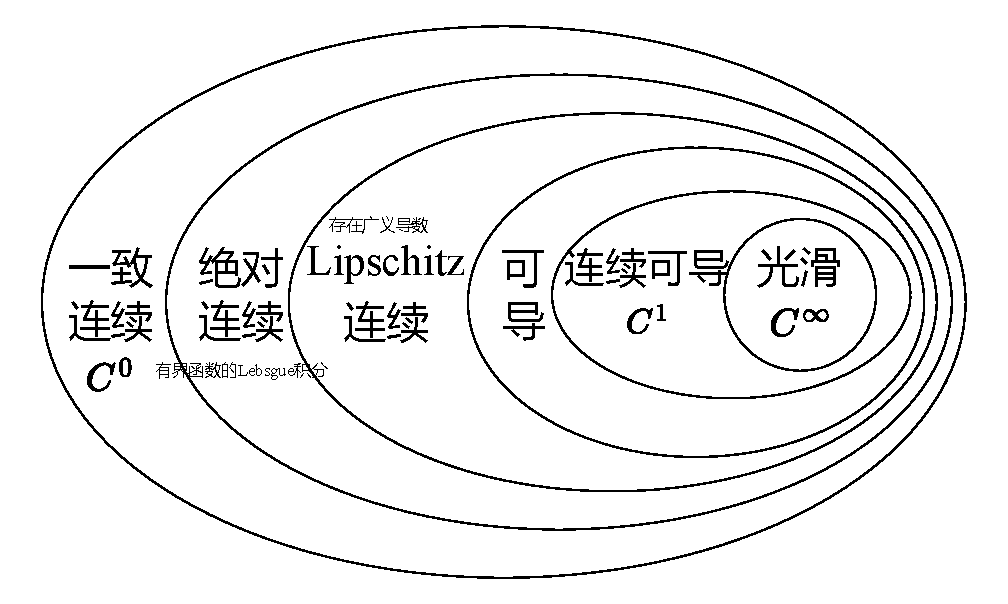
\includegraphics[width=0.6\linewidth]{asserts/连续的关系.drawio.pdf}
  \caption{控制理论中常用的连续性质的关系}
  \label{fig continuity}
\end{figure}


如下绝对值函数\(f_2(x)\)绝对连续但是在0处不连续可微 \[
f_2(x)=|x|, x\in [-1,1]
\]

如下根号函数绝对连续但是在0处不是局部Lipschitz连续的 \[
f_3(t)=\sqrt(t),t\in [0,0]
\]

\section{连续可微和光滑}

连续可微(Continuously differentiable),用泛函表示就是函数\(f\in C^1\),意味着函数的导数是连续的,当然可微保证其本身也是连续的。

光滑函数(英语:Smooth function)在数学中特指无穷可导的函数,不存在尖点,也就是说所有的有限阶导数都存在。例如,指数函数就是光滑的,因为指数函数的导数是指数函数本身。

\begin{definition}[光滑函数]
  若一函数是连续的,则称其为\(C^{0}\)函数;
  若函数存在导函数,且其导函数连续,则称为连续可导,记为\(C^1\)函数;
  若一函数n阶可导,并且其n阶导函数连续,则为\(C^{n}\)函数(\(n\geq 1\))。
  而光滑函数是对所有n都属于\(C^{n}\)函数,特称其为\(C^{\infty }\)函数。
\end{definition}


\section{内容概要}

从这个图可以看出在经典解中解$x(t)$是$f(x(t))$的积分,而Filippov解中$x(t)$是$f(x(t))$的Lebsgue积分。
经典解中的解是连续可导的,连续可导的意思是可导并且其导数连续,这与存在性条件$f(x(t))$连续一致。
类似地,Filippov解中解是绝对连续的,这与存在性条件$f(x(t))$可测并且局部本质有界一致。

\begin{table}[!htp]
  \centering
  \begin{tabular}{|c|c|c|c|}
    \hline
    & 解$x(t)$的连续性 & 存在性条件 & 唯一性条件 \\\hline
    经典解 & 连续可导 & 
    $f(x)$连续 & $f(x)$ Lipschitz连续\\\hline
    Filippov解 & 绝对连续 & 
    $f(x)$ 可测并且局部本质有界 & $f(x)$ Lipschitz连续 \\\hline
  \end{tabular}
  \caption{微分方程$\dot{x}=f(x)$Filippov解}
\end{table}

Every vector field that is locally Lipschitz at $x$ satisfies the one-sided Lipschitz condition on a neighborhood of $x$, but the converse is not true.
